\documentclass[landscape,final,paperwidth=48in,paperheight=33in,fontscale=0.285]{baposter}
%\usepackage{calc,array}
\usepackage{graphicx} % Required for including images
\usepackage{amsmath}  % For typesetting math
\usepackage{amssymb}  % Adds new symbols to be used in math mode
\usepackage{relsize}  % Chagnge size of text /smaller, /larger
\usepackage{multirow} % Allows table cells to span more than one row of the table
\usepackage{rotating} % Rotate figures and tables
\usepackage{bm}       % Allows a math expression to be bold
\usepackage{url}      % Allows email address and websites
\usepackage{gensymb}  % Allows degree symbol
\usepackage{siunitx}  % Scientific notation

\usepackage{float}
\usepackage{caption} % Required for specifying captions to tables and figures
\usepackage{wrapfig} % Wrap text around figure
\usepackage[export]{adjustbox}

%\captionsetup[figure]{font=Large,skip=0pt,labelformat=empty,justification=raggedright,singlelinecheck=false}

\usepackage{multicol} % Required for multiple columns

\usepackage[utf8]{inputenc} %Required for IEEE reference style
\newcommand{\BIBdecl}{\setlength{\itemsep}{-0.25 em}} %Removes line space between references

% Fonts
%\usepackage{times}
%\usepackage{helvet}
%\usepackage{bookman}
\usepackage{palatino}

%\newcommand{\captionfont}{\footnotesize}

\graphicspath{{../../group-analysis-child_files/figure-html}{img/}}
%\usetikzlibrary{calc}

\newcommand{\SET}[1]  {\ensuremath{\mathcal{#1}}}
\newcommand{\MAT}[1]  {\ensuremath{\boldsymbol{#1}}}
\newcommand{\VEC}[1]  {\ensuremath{\boldsymbol{#1}}}
\newcommand{\Video}{\SET{V}}
\newcommand{\video}{\VEC{f}}
\newcommand{\track}{x}
\newcommand{\Track}{\SET T}
\newcommand{\LMs}{\SET L}
\newcommand{\lm}{l}
\newcommand{\PosE}{\SET P}
\newcommand{\posE}{\VEC p}
\newcommand{\negE}{\VEC n}
\newcommand{\NegE}{\SET N}
\newcommand{\Occluded}{\SET O}
\newcommand{\occluded}{o}

%%%%%%%%%%%%%%%%%%%%%%%%%%%%%%%%%%%%%%%%%%%%%%%%%%%%%%%%%%%%%%%%%%%%%%%%%%%%%%%%
% Multicol Settings
%%%%%%%%%%%%%%%%%%%%%%%%%%%%%%%%%%%%%%%%%%%%%%%%%%%%%%%%%%%%%%%%%%%%%%%%%%%%%%%%
\setlength{\columnsep}{1.5em}
\setlength{\columnseprule}{0mm}
%%%%%%%%%%%%%%%%%%%%%%%%%%%%%%%%%%%%%%%%%%%%%%%%%%%%%%%%%%%%%%%%%%%%%%%%%%%%%%%%
% Save space in lists. Use this after the opening of the list
%%%%%%%%%%%%%%%%%%%%%%%%%%%%%%%%%%%%%%%%%%%%%%%%%%%%%%%%%%%%%%%%%%%%%%%%%%%%%%%%
\newcommand{\compresslist}{%
\setlength{\itemsep}{1pt}%
\setlength{\parskip}{0pt}%
\setlength{\parsep}{0pt}%
}
%%%%%%%%%%%%%%%%%%%%%%%%%%%%%%%%%%%%%%%%%%%%%%%%%%%%%%%%%%%%%%%%%%%%%%%%%%%%%%
%%% Begin of Document
%%%%%%%%%%%%%%%%%%%%%%%%%%%%%%%%%%%%%%%%%%%%%%%%%%%%%%%%%%%%%%%%%%%%%%%%%%%%%%

\begin{document}

%%%%%%%%%%%%%%%%%%%%%%%%%%%%%%%%%%%%%%%%%%%%%%%%%%%%%%%%%%%%%%%%%%%%%%%%%%%%%%
%%% Here starts the poster
%%%---------------------------------------------------------------------------
%%% Format it to your taste with the options
%%%%%%%%%%%%%%%%%%%%%%%%%%%%%%%%%%%%%%%%%%%%%%%%%%%%%%%%%%%%%%%%%%%%%%%%%%%%%%
% Define some colors

%\definecolor{lightblue}{cmyk}{0.83,0.24,0,0.12}
\definecolor{lightblue}{rgb}{0.145,0.6666,1}

%\newtcolorbox{demobox}[1][]{colback=white,colframe=lightblue,width=0.33\linewidth,nobeforeafter,box align=top,before=\noindent,#1}

%%
\begin{poster}%
  % Poster Options
  {
  % Show grid to help with alignment
  grid=false,
  % Column spacing
  colspacing=1em,
  % Color style
  bgColorOne=white,
  bgColorTwo=white,
  borderColor=lightblue,
  headerColorOne=black,
  headerColorTwo=lightblue,
  headerFontColor=white,
  boxColorOne=white,
  boxColorTwo=lightblue,
  % Format of textbox
  textborder=roundedleft,
  % Format of text header
  eyecatcher=true,
  headerborder=closed,
  headerheight=0.12\textheight,
  columns=4, %default=4 for landscape posters maximum columns=6
%  textfont=\sc, An example of changing the text font
  headershape=roundedright,
  headershade=shadelr,
  headerfont=\Large\bf\textsc, %Sans Serif
  textfont={\setlength{\parindent}{1.5em}},
  boxshade=plain,
%  background=shade-tb,
  background=plain,
  linewidth=2pt
  }
  % University logo
  {
\includegraphics[height=6em]{penn_state_cla_logo_new_210-89.jpg}}
  % Title
  {\vspace{0.1em}
  \bf{Infant brain responses differentiate between optic flow\\ patterns and motion speeds} 
  \vspace{0.3em}}
  % Authors
  {Alyssa Pandos \emph{(aap5371@psu.edu)}, Rick O. Gilmore, and Andrea R. Seisler\\ \vspace{0.3em}
  }
  % Databrary Logo
 {
\includegraphics[height=4em]{databrary.png}}

%%%%%%%%%%%%%%%%%%%%%%%%%%%%%%%%%%%%%%%%%%%%%%%%%%%%%%%%%%%%%%%%%%%%%%%%%%%%%%
%%% Now define the boxes that make up the poster
%%%---------------------------------------------------------------------------
%%% Each box has a name and can be placed absolutely or relatively.
%%% The only inconvenience is that you can only specify a relative position
%%% towards an already declared box. So if you have a box attached to the
%%% bottom, one to the top and a third one which should be in between, you
%%% have to specify the top and bottom boxes before you specify the middle
%%% box.
%%%%%%%%%%%%%%%%%%%%%%%%%%%%%%%%%%%%%%%%%%%%%%%%%%%%%%%%%%%%
%
%%%%%%%%%%%%%%%%%%%%%%%%%%%%%%%%%%%%%%%%%%%%%%%%%%%%%%%%%%%%%%%%%%%%%%%%%%%%%%
\headerbox{Background}{name=background,column=0,span=1,row=0}
%%%%%%%%%%%%%%%%%%%%%%%%%%%%%%%%%%%%%%%%%%%%%%%%%%%%%%%%%%%%%%%%%%%%%%%%%%%%%%
    {
    Optic flow informs infants' perception of the geometry, speed, and motion of objects in their environment and their own movements through space. Prior research suggests that infants show larger amplitude electroencephalographic (EEG) responses to direction-reversing linear patterns of optic flow \cite{Gilmore2007-od} than to radial or rotational patterns. Infants also show larger EEG responses to coherence-modulating rotational flow patterns when motion speeds are faster \cite{Hou2009-iz}. Moreover, children 4-8 years old show larger amplitude EEG responses to fast radial and rotational optic flow \cite{Gilmore2016-sd}, suggesting that the motion processing network undergoes prolonged development throughout childhood.
    }
%%%%%%%%%%%%%%%%%%%%%%%%%%%%%%%%%%%%%%%%%%%%%%%%%%%%%%%%%%%%%%%%%%%%%%%%%%%%%%
\headerbox{Methods}{name=methods,column=0,span = 1,below=background}
%%%%%%%%%%%%%%%%%%%%%%%%%%%%%%%%%%%%%%%%%%%%%%%%%%%%%%%%%%%%%%%%%%%%%%%%%%%%%%
    {
\par To provide a direct comparison with prior child neural data, high density (128 channel) EEG responses were recorded from (n=23; 13 female) 17- to 38-week-old infants who viewed two different patterns (radial and linear) of optic flow presented at two different speeds (2 and 8 deg/s). Flow patterns were generated from white dots moving on a black background, with the degree of motion coherence varying from 100 percent (coherent) to 0 percent (incoherent/random) every 833 ms, resulting in a first harmonic (1F1) of 1.2 Hz. EEG data were cleaned and filtered before being subjected to a frequency domain analysis using a discrete Fourier transform. This analysis provided data about complex domain responses to the optic flow stimulus at low-order integer harmonics of the coherence modulating frequency (e.g., 1F1, 2F1, 3F1).
    }
%%%%%%%%%%%%%%%%%%%%%%%%%%%%%%%%%%%%%%%%%%%%%%%%%%%%%%%%%%%%%%%%%%%%%%%%%%%%%%
\headerbox{Displays}{name=displays, column=1, span=1, row=0}
%%%%%%%%%%%%%%%%%%%%%%%%%%%%%%%%%%%%%%%%%%%%%%%%%%%%%%%%%%%%%%%%%%%%%%%%%%%%%%
    {
\begin{center}

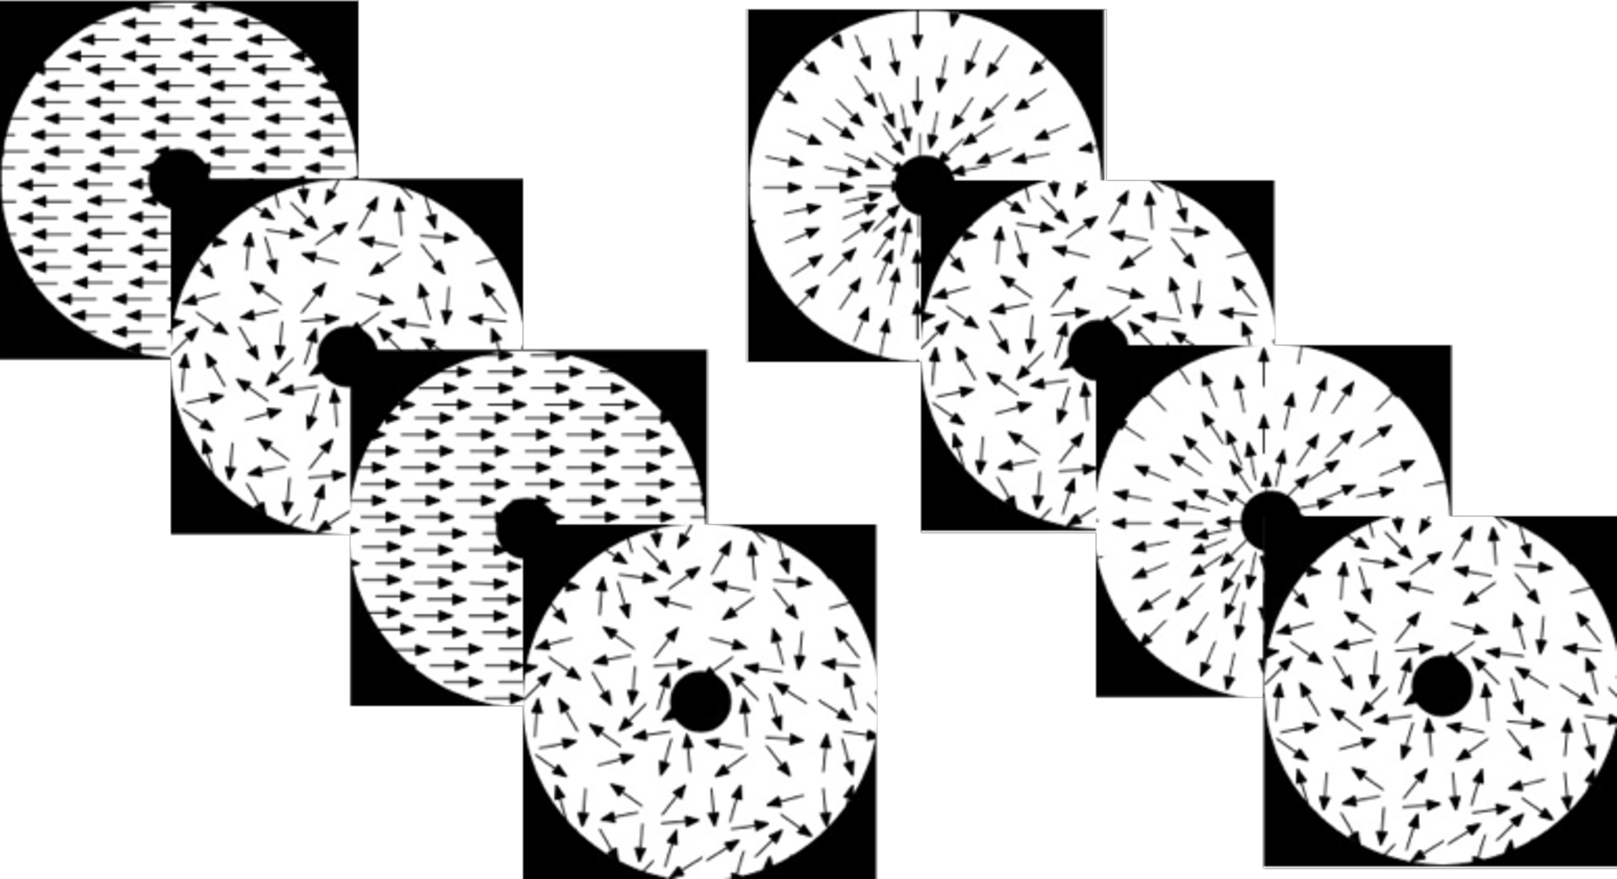
\includegraphics[scale=0.1, height=40mm]{FINAL-DISPLAYS.pdf}

\end{center}

}
%%%%%%%%%%%%%%%%%%%%%%%%%%%%%%%%%%%%%%%%%%%%%%%%%%%%%%%%%%%%%%%%%%%%%%%%%%%%%%
\headerbox{Results and Discussion}{name=stats, column=1, span=1, below=displays}
%%%%%%%%%%%%%%%%%%%%%%%%%%%%%%%%%%%%%%%%%%%%%%%%%%%%%%%%%%%%%%%%%%%%%%%%%%%%%%
    {
\par At the first harmonic, infants showed a small cluster of left frontal channels that showed higher amplitude responses to translational patterns and a larger cluster over the posterior midline that showed higher amplitude and distinct phase responses to faster speeds. At the second harmonic (2F1; 2.4 Hz), there was a cluster of left frontal channels that showed higher amplitudes to radial motion, a group of left lateral channels that showed higher amplitudes to faster speeds, and a right lateral cluster that showed a pattern by speed interaction. Results from the third harmonic (not shown) showed a small left frontal cluster of channels with higher responses to radial motion and two left and right central clusters where EEG phases, amplitudes, or both distinguished between the two speed conditions.

Taken together, the results show that infant brain responses to coherence-modulating optic flow differ both from prior EEG results using direction-changing optic flows \cite{Gilmore2007-od} and from those recorded in older children using identical displays \cite{Gilmore2016-sd}. Faster (8 deg/s vs. 2 deg/s) speeds tend to evoke larger amplitude EEG responses, consistent with predictions, but radial flows activated larger amplitude responses than linear flows, in contrast with predictions. Moreover, the spatial pattern of channels showing speed or pattern sensitivity differs between infants, children, and adults. The network of brain systems that detect and respond to optic flow may undergo patterns of development that are more idiosyncratic or individual-specific than indicated by previous findings.

}
%%%%%%%%%%%%%%%%%%%%%%%%%%%%%%%%%%%%%%%%%%%%%%%%%%%%%%%%%%%%%%%%%%%%%%%%%%%%%%
\headerbox{Results: 1F1}{name=graphs1, column=2, row=0, span=1}
%%%%%%%%%%%%%%%%%%%%%%%%%%%%%%%%%%%%%%%%%%%%%%%%%%%%%%%%%%%%%%%%%%%%%%%%%%%%%%
    {
 \begin{center}

 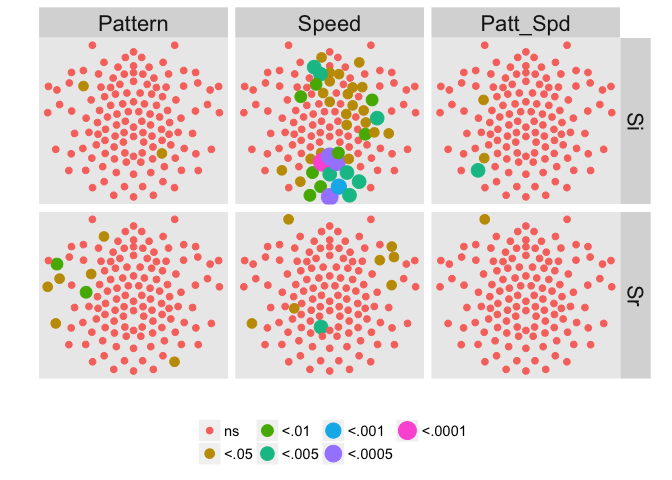
\includegraphics[scale=0.3,valign=t]{channel-effects-plot-1.png}
 
 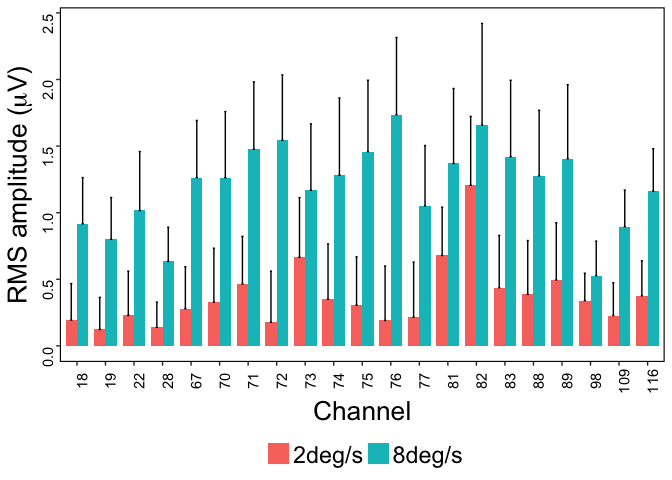
\includegraphics[scale=0.3,valign=t]{figX-vector-amplitude-barplots-speed-1-1F1.png}
 
 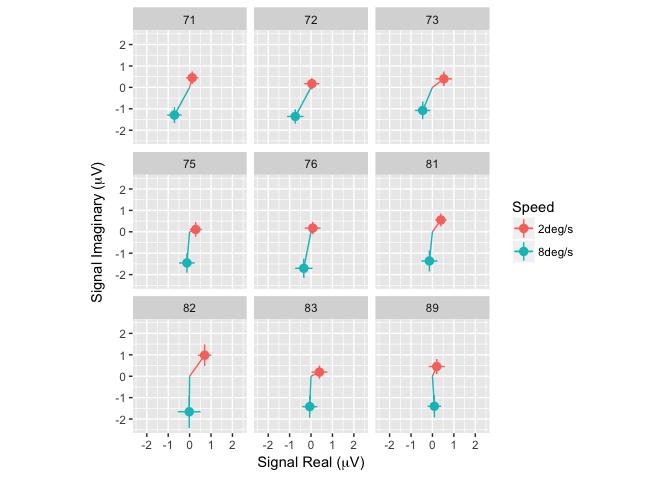
\includegraphics[scale=0.3,valign=t]{figX-complex-domain-speed-1.png}
 \end{center}
 }

%%%%%%%%%%%%%%%%%%%%%%%%%%%%%%%%%%%%%%%%%%%%%%%%%%%%%%%%%%%%%%%%%%%%%%%%%%%%%%
\headerbox{Results: 2F1}{name=graphs2, column=3, row=0, span=1}
%%%%%%%%%%%%%%%%%%%%%%%%%%%%%%%%%%%%%%%%%%%%%%%%%%%%%%%%%%%%%%%%%%%%%%%%%%%%%%
    {
 \begin{center}

 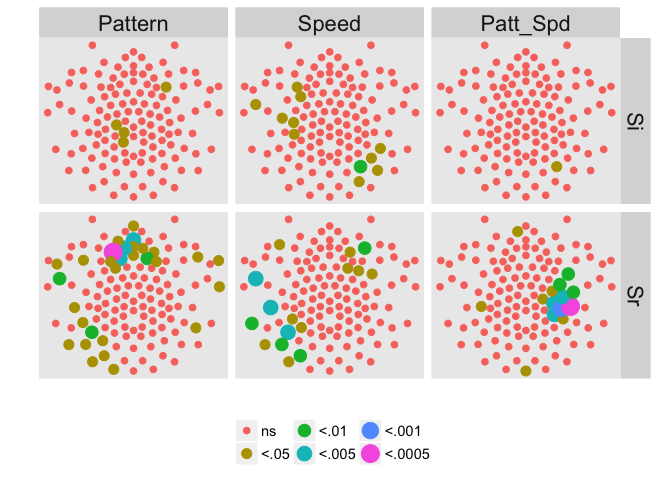
\includegraphics[scale=0.3,valign=t]{channel-effects-plot-2F1.png}
 
  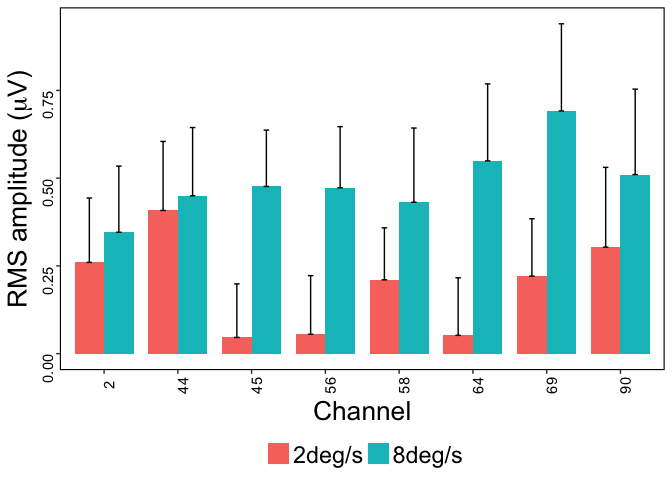
\includegraphics[scale=0.3,valign=t]{figX-vector-amplitude-barplots-speed-1-2F1.png}

 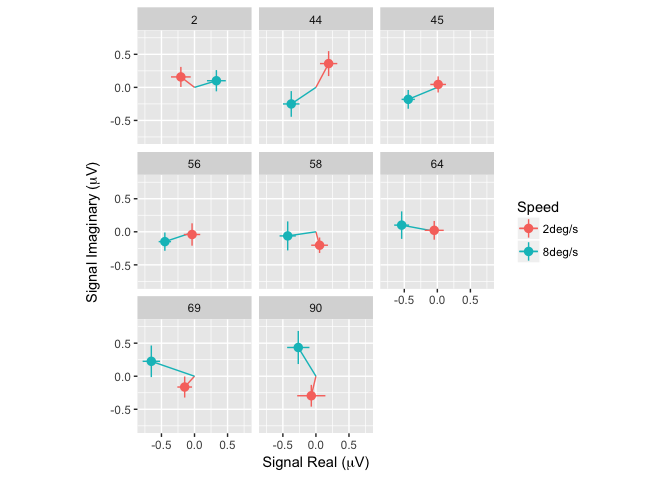
\includegraphics[scale=0.3,valign=t]{figX-complex-domain-speed-1-2F1.png}
 \end{center}
}

%%%%%%%%%%%%%%%%%%%%%%%%%%%%%%%%%%%%%%%%%%%%%%%%%%%%%%%%%%%%%%%%%%%%%%%%%%%%%%
  \headerbox{Acknowledgements}{name=thanks, column=2, below=graphs1, above=bottom}
%%%%%%%%%%%%%%%%%%%%%%%%%%%%%%%%%%%%%%%%%%%%%%%%%%%%%%%%%%%%%%%%%%%%%%%%%%%%%%
    {
   \smaller
   
      This material is based upon work supported by the National Science Foundation under Grant Number BCS-1147440.
      Any opinions, findings, and conclusions or recommendations expressed in this material are those of the author(s) and do not necessarily reflect the views of the National Science Foundation.
    }
%%%%%%%%%%%%%%%%%%%%%%%%%%%%%%%%%%%%%%%%%%%%%%%%%%%%%%%%%%%%%%%%%%%%%%%%%%%%%%
   \headerbox{Data Sharing}{name=sharing, column=3, below=graphs2, above=bottom}
%%%%%%%%%%%%%%%%%%%%%%%%%%%%%%%%%%%%%%%%%%%%%%%%%%%%%%%%%%%%%%%%%%%%%%%%%%%%%%%
    {
    \smaller
    
       Movies of the displays, metadata about the participants, and raw data files are available at: \url{http://databrary.org/volume/218}. Full reports of our data analysis workflows are available at: \url{http://github.com/gilmore-lab/moco-psychophysics/child-laminar-radial}
       
       }

%%%%%%%%%%%%%%%%%%%%%%%%%%%%%%%%%%%%%%%%%%%%%%%%%%%%%%%%%%%%%%%%%%%%%%%%%%%%%%
 \headerbox{References}{name=refs, column=0, span=1, below=methods, above=bottom}
%%%%%%%%%%%%%%%%%%%%%%%%%%%%%%%%%%%%%%%%%%%%%%%%%%%%%%%%%%%%%%%%%%%%%%%%%%%%%%
  {
  %For use with external .bib file
  
  \tiny
  
          \renewcommand{\refname}{\vspace{-0.5em}} % removes "References" canned text.
          \bibliographystyle{IEEEtran}
          \bibliography{IEEEabrv,poster_landscape}
          
}
\end{poster}
\end{document}
